% Created by tikzDevice version 0.12.5 on 2024-01-27 23:38:32
% !TEX encoding = UTF-8 Unicode
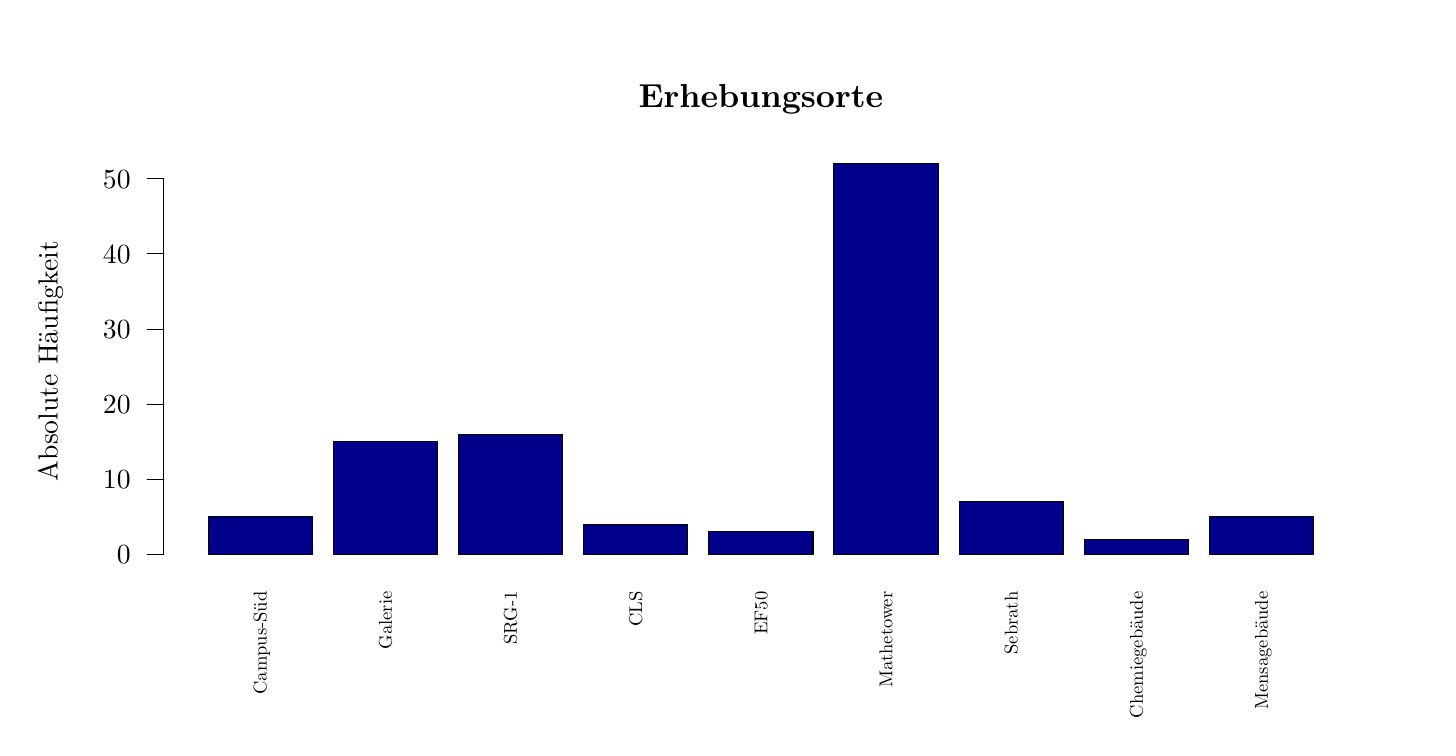
\begin{tikzpicture}[x=1pt,y=1pt]
\definecolor{fillColor}{RGB}{255,255,255}
\path[use as bounding box,fill=fillColor,fill opacity=0.00] (0,0) rectangle (505.89,252.94);
\begin{scope}
\path[clip] (  0.00,  0.00) rectangle (505.89,252.94);
\definecolor{drawColor}{RGB}{0,0,0}
\definecolor{fillColor}{RGB}{0,0,139}

\path[draw=drawColor,line width= 0.4pt,line join=round,line cap=round,fill=fillColor] ( 65.18, 62.61) rectangle (102.87, 76.18);

\path[draw=drawColor,line width= 0.4pt,line join=round,line cap=round,fill=fillColor] (110.41, 62.61) rectangle (148.10,103.32);

\path[draw=drawColor,line width= 0.4pt,line join=round,line cap=round,fill=fillColor] (155.64, 62.61) rectangle (193.33,106.04);

\path[draw=drawColor,line width= 0.4pt,line join=round,line cap=round,fill=fillColor] (200.87, 62.61) rectangle (238.56, 73.47);

\path[draw=drawColor,line width= 0.4pt,line join=round,line cap=round,fill=fillColor] (246.10, 62.61) rectangle (283.79, 70.75);

\path[draw=drawColor,line width= 0.4pt,line join=round,line cap=round,fill=fillColor] (291.33, 62.61) rectangle (329.02,203.75);

\path[draw=drawColor,line width= 0.4pt,line join=round,line cap=round,fill=fillColor] (336.56, 62.61) rectangle (374.25, 81.61);

\path[draw=drawColor,line width= 0.4pt,line join=round,line cap=round,fill=fillColor] (381.79, 62.61) rectangle (419.48, 68.04);

\path[draw=drawColor,line width= 0.4pt,line join=round,line cap=round,fill=fillColor] (427.02, 62.61) rectangle (464.71, 76.18);
\end{scope}
\begin{scope}
\path[clip] (  0.00,  0.00) rectangle (505.89,252.94);
\definecolor{drawColor}{RGB}{0,0,0}

\node[text=drawColor,rotate= 90.00,anchor=base east,inner sep=0pt, outer sep=0pt, scale=  0.67] at ( 86.33, 49.20) {Campus-Süd};

\node[text=drawColor,rotate= 90.00,anchor=base east,inner sep=0pt, outer sep=0pt, scale=  0.67] at (131.56, 49.20) {Galerie};

\node[text=drawColor,rotate= 90.00,anchor=base east,inner sep=0pt, outer sep=0pt, scale=  0.67] at (176.79, 49.20) {SRG-1};

\node[text=drawColor,rotate= 90.00,anchor=base east,inner sep=0pt, outer sep=0pt, scale=  0.67] at (222.02, 49.20) {CLS};

\node[text=drawColor,rotate= 90.00,anchor=base east,inner sep=0pt, outer sep=0pt, scale=  0.67] at (267.25, 49.20) {EF50};

\node[text=drawColor,rotate= 90.00,anchor=base east,inner sep=0pt, outer sep=0pt, scale=  0.67] at (312.48, 49.20) {Mathetower};

\node[text=drawColor,rotate= 90.00,anchor=base east,inner sep=0pt, outer sep=0pt, scale=  0.67] at (357.71, 49.20) {Sebrath};

\node[text=drawColor,rotate= 90.00,anchor=base east,inner sep=0pt, outer sep=0pt, scale=  0.67] at (402.94, 49.20) {Chemiegebäude};

\node[text=drawColor,rotate= 90.00,anchor=base east,inner sep=0pt, outer sep=0pt, scale=  0.67] at (448.17, 49.20) {Mensagebäude};
\end{scope}
\begin{scope}
\path[clip] (  0.00,  0.00) rectangle (505.89,252.94);
\definecolor{drawColor}{RGB}{0,0,0}

\node[text=drawColor,anchor=base,inner sep=0pt, outer sep=0pt, scale=  1.20] at (264.94,224.20) {\bfseries Erhebungsorte};

\node[text=drawColor,rotate= 90.00,anchor=base,inner sep=0pt, outer sep=0pt, scale=  1.00] at ( 10.80,132.47) {Absolute Häufigkeit};
\end{scope}
\begin{scope}
\path[clip] (  0.00,  0.00) rectangle (505.89,252.94);
\definecolor{drawColor}{RGB}{0,0,0}

\path[draw=drawColor,line width= 0.4pt,line join=round,line cap=round] ( 49.20, 62.61) -- ( 49.20,198.32);

\path[draw=drawColor,line width= 0.4pt,line join=round,line cap=round] ( 49.20, 62.61) -- ( 43.20, 62.61);

\path[draw=drawColor,line width= 0.4pt,line join=round,line cap=round] ( 49.20, 89.75) -- ( 43.20, 89.75);

\path[draw=drawColor,line width= 0.4pt,line join=round,line cap=round] ( 49.20,116.89) -- ( 43.20,116.89);

\path[draw=drawColor,line width= 0.4pt,line join=round,line cap=round] ( 49.20,144.03) -- ( 43.20,144.03);

\path[draw=drawColor,line width= 0.4pt,line join=round,line cap=round] ( 49.20,171.18) -- ( 43.20,171.18);

\path[draw=drawColor,line width= 0.4pt,line join=round,line cap=round] ( 49.20,198.32) -- ( 43.20,198.32);

\node[text=drawColor,anchor=base east,inner sep=0pt, outer sep=0pt, scale=  1.00] at ( 37.20, 59.17) {0};

\node[text=drawColor,anchor=base east,inner sep=0pt, outer sep=0pt, scale=  1.00] at ( 37.20, 86.31) {10};

\node[text=drawColor,anchor=base east,inner sep=0pt, outer sep=0pt, scale=  1.00] at ( 37.20,113.45) {20};

\node[text=drawColor,anchor=base east,inner sep=0pt, outer sep=0pt, scale=  1.00] at ( 37.20,140.59) {30};

\node[text=drawColor,anchor=base east,inner sep=0pt, outer sep=0pt, scale=  1.00] at ( 37.20,167.73) {40};

\node[text=drawColor,anchor=base east,inner sep=0pt, outer sep=0pt, scale=  1.00] at ( 37.20,194.87) {50};
\end{scope}
\end{tikzpicture}
